% LaTeX Präsentationsvorlage (2013) der TU Graz, rev12, 2013/01/31
% !TeX encoding = UTF-8
\documentclass{beamer}
% \documentclass[aspectratio=169]{beamer}
% \usetheme{tugraz2013}
% \usetheme[notes]{tugraz2013}
\usepackage{../common/beamerthemetugraz2013}
\usepackage{color}
\usepackage{multicol}
\usepackage{bbding}
\usepackage{wasysym}
\usepackage{caption}
% \usepackage{minted}

\usepackage{listings}
\usepackage{xcolor}

\definecolor{codegreen}{rgb}{0,0.6,0}
\definecolor{codegray}{rgb}{0.5,0.5,0.5}
\definecolor{codepurple}{rgb}{0.58,0,0.82}
\definecolor{backcolour}{rgb}{0.95,0.95,0.92}
\lstdefinestyle{mystyle}{
    backgroundcolor=\color{backcolour},   
    commentstyle=\color{codegreen},
    keywordstyle=\color{magenta},
    numberstyle=\tiny\color{codegray},
    stringstyle=\color{codepurple},
    basicstyle=\ttfamily\footnotesize,
    breakatwhitespace=false,         
    breaklines=true,                 
    captionpos=b,                    
    keepspaces=true,                 
    numbers=left,                    
    numbersep=5pt,                  
    showspaces=false,                
    showstringspaces=false,
    showtabs=false,                  
    tabsize=2
}

\lstset{style=mystyle}

\usepackage{picture}
\usepackage{rotating}

\definecolor{darkred}{rgb}{0.85,0.16,0.0}
\definecolor{darkgreen}{rgb}{0.16,0.70,0.27}

\newcommand{\hrefu}[2]{\underline{\href{#1}{#2}}}

\newcommand{\red}[1]{{\color{red} #1}}
\newcommand{\blue}[1]{{\color{blue} #1}}
\newcommand{\darkgreen}[1]{\textcolor{darkgreen}{#1}}
\newcommand{\darkred}[1]{\textcolor{darkred}{#1}}

\newcommand*{\vpointer}{\vcenter{\hbox{\scalebox{1.5}{\large\pointer}}}}

%% Titelblatt-Einstellungen
\title[]
{Python 03}
\author[E.~Wachmann]{\scriptsize Elias Wachmann
}
\date{2024} % \today für heutiges Datum verwenden
\institute[Institute of Theoretical and Computational Physics]
{
}
\instituteurl{www.tugraz.at}
% \institutelogo{kurz.pdf}
%~ \additionallogo{merged_logos}
\AtBeginSection[]{
  \begin{frame}
  \vfill
  \centering
  \begin{beamercolorbox}[sep=8pt,center,shadow=true,rounded=true]{title}
    \usebeamerfont{title}\insertsectionhead\par%
  \end{beamercolorbox}
  \vfill
  \end{frame}
}
%%%%%%%%%%%%%%%%%%%%%%%%%%%%%%%%%%%%%%%%%%%%%%%%%%%%%%%%%%%%%%%%%%%%%%%%%%%%
\begin{document}
%%%%%%%%%%%%%%%%%%%%%%%%%%%%%%%%%%%%%%%%%%%%%%%%%%%%%%%%%%%%%%%%%%%%%%%%%%%%
\titleframe

%\begin{frame}
%  \frametitle{Outline}
%  \tableofcontents%[hideallsubsections] 
%  \note{
%  	Meine Präsentation ist wie folgt strukturiert \ldots
%  }
%\end{frame}

\section*{Content}
\begin{frame}
\frametitle{Content}
  \tableofcontents
\end{frame}

\section{Variables}

\begin{frame}
\frametitle{Variable Names}
  From \href[]{https://peps.python.org/pep-0008/}{PEP-8 Style Guide}:
  \begin{itemize}
    \item must start with letter or \_
    \item can only contain alpha-numeric values (a-z, A-Z, 0-9) and \_
    \item variable names are case sensitive
    \item do not overwrite built-in functions 
  \end{itemize}
\end{frame}

\begin{frame}
  \frametitle{Naming conventions}
    According to \href[]{https://peps.python.org/pep-0008/}{PEP-8 Style Guide}:
    \begin{itemize}
      \item CONST\_NAMES are all caps with \_ between words
      \item function\_names are all lower case with \_ between words
      \item variables follow the same rules as functions
      \item ClassNames are CamelCase
    \end{itemize}
  \end{frame}
\section{Python files}

\begin{frame}
\frametitle{Python files and usage}
  \begin{itemize}
    \item Python files are called \texttt{.py}
    \item Python files can be run from the command line
    \begin{itemize}
      \item \texttt{python3 file.py}
    \end{itemize} 
    \item Python files can be imported into other Python files
    \begin{itemize}
      \item \texttt{import numpy}
      \item or with an alias \texttt{import numpy as np}
    \end{itemize}
    \item Python files can be run as scripts or imported as modules
  \end{itemize}
\end{frame}
\begin{frame}
  \frametitle{Python files run as scripts}
  I can simply run this file and it will print the sinus values from y for the indices 5 through 10 (excluding 10).
  \lstinputlisting[language=python]{examples/myscript.py}
  What happens if I import this file in another file?
\end{frame}
\begin{frame}
  \frametitle{Python files imported as modules}
  I can now import myscript.py in another file using the \texttt{import} statement:
  \lstinputlisting[language=python]{examples/import.py}
  \vspace{5mm}
  What happens if I run this file?
\end{frame}
\begin{frame}
  \frametitle{Python files imported as modules}
  \begin{figure}[H]
    \includegraphics[width=\textwidth]{fig/output\_import.png}
  \end{figure}
  It not only prints the \textit{This is import.py} line, but also the sinus values from y for the indices 5 through 10 (excluding 10).\\
  These are printed because the \texttt{import} statement runs the file as a script.\\
  How to avoid this?
\end{frame}
\begin{frame}
  \frametitle{\_\_name\_\_ == '\_\_main\_\_'}
  By using the \texttt{\_\_name\_\_} variable, we can avoid running the file as a script when it is imported as a module.\\
  \vspace{5mm}
  \lstinputlisting[language=python]{examples/myscript2.py}
  Importing this file in another file will not print the sinus values.
\end{frame}



\section{Functions}
\begin{frame}
  \frametitle{Functions}
  \begin{itemize}
    \item Functions are defined with \texttt{def}
    \item Functions can have arguments
    \item Functions can return values
    \item Functions can have default arguments
    \item Functions can have variable number of arguments
  \end{itemize}
\end{frame}

\begin{frame}
  \frametitle{Some examples}
  \lstinputlisting[language=python, firstline=1,lastline=10]{examples/functions.py}
\end{frame}
\begin{frame}
  \frametitle{Some examples}
  \lstinputlisting[language=python, firstline=13]{examples/functions.py}
\end{frame}
\begin{frame}
  \frametitle{Multi returns}
  Multiple returns from the same funciton
  \lstinputlisting[language=python]{examples/multireturn.py}
\end{frame}
\begin{frame}
  \frametitle{Import functions from other files}
  \lstinputlisting[language=python]{examples/myfunc.py}
  \vspace{5mm}
  Import the functions from myfunc.py in another file (just like we did with numpy):
  \lstinputlisting[language=python]{examples/myimport.py}
\end{frame}
\section{Fitting Data}
\begin{frame}
  \frametitle{Fitting Data}
  In physics we often have to fit data to a function. \\ There are many ways to fit a function to given data. For now we will use \hrefu{https://numpy.org/}{numpy's} \hrefu{https://numpy.org/doc/stable/reference/generated/numpy.polyfit.html}{\texttt{polyfit()}} function.\\ \vspace{5mm}
  It fits a polynomial of degree \texttt{deg} to the data reducing the sum of squared residuals.\\ It returns the coefficients of the polynomial in decreasing powers.\\
\end{frame}

\begin{frame}
  \frametitle{Fitting Data - Experimental Data}
  From our measurements we get the following data:
  \begin{figure}[H]
    \centering
    \begin{samepage}
        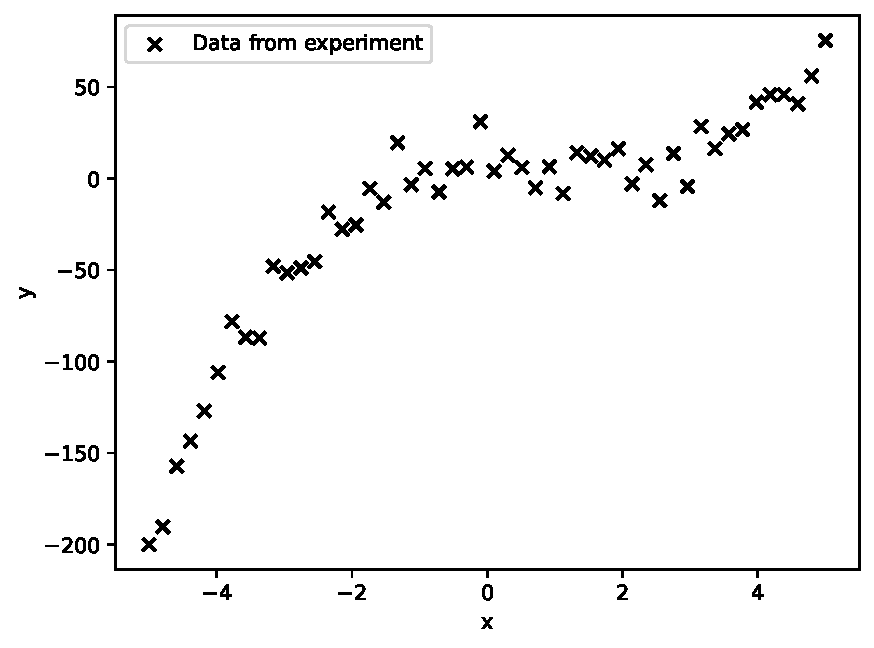
\includegraphics[width=0.65\linewidth]{fig/fitting1.pdf}
    \end{samepage}
\end{figure}
\end{frame}

\begin{frame}
  \frametitle{Fitting Data - Linear Fit}
  \lstinputlisting[language=python, firstline=4, lastline=12]{examples/fitting2.py}
  \hrefu{https://numpy.org/doc/stable/reference/generated/numpy.polyval.html}{\texttt{polyval()}} evaluates the polynomial at the given points.
\end{frame}

\begin{frame}
  \frametitle{Fitting - Linear Fit}
  \begin{minipage}[t]{0.25\textwidth}
    \vspace{-5.0cm}
    A linear fit on the data works well for $x \in [-2,3]$, but not outside this range.
\end{minipage}
\hfill
\begin{minipage}[t]{0.72\textwidth}
    \centering
    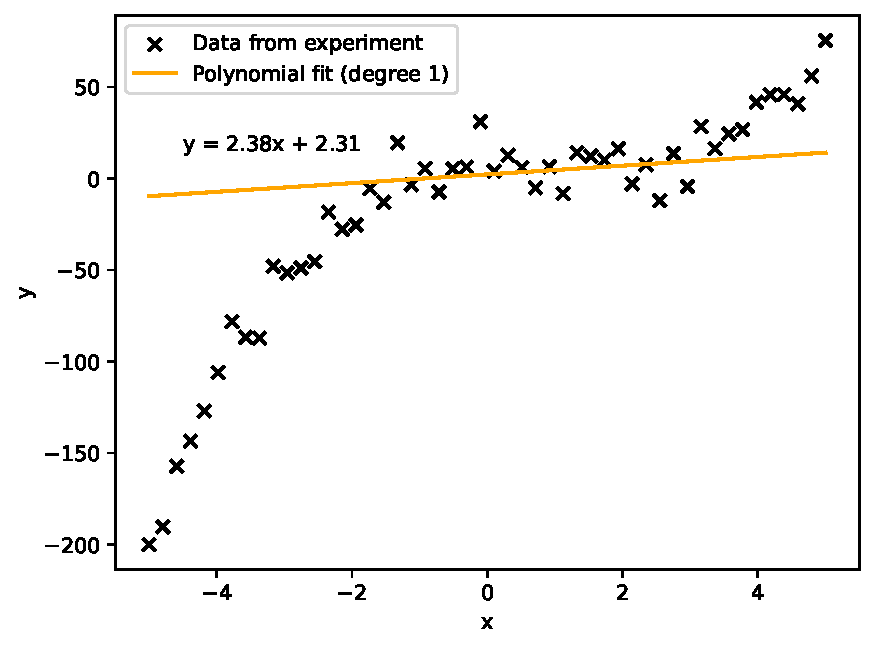
\includegraphics[width=\linewidth]{fig/fitting2.pdf}
\end{minipage}
\end{frame}

\begin{frame}
  \frametitle{Fitting Data - Cubic Fit}
  We can now add another fit, this time a cubic fit:
  \lstinputlisting[language=python, firstline=13]{examples/fitting2.py}
  
\end{frame}

\begin{frame}
  \frametitle{Fitting - Cubic Fit}
  \begin{minipage}[t]{0.25\textwidth}
    \vspace{-5.0cm}
    A cubic fit describes the data better than a linear fit.
\end{minipage}
\hfill
\begin{minipage}[t]{0.72\textwidth}
    \centering
    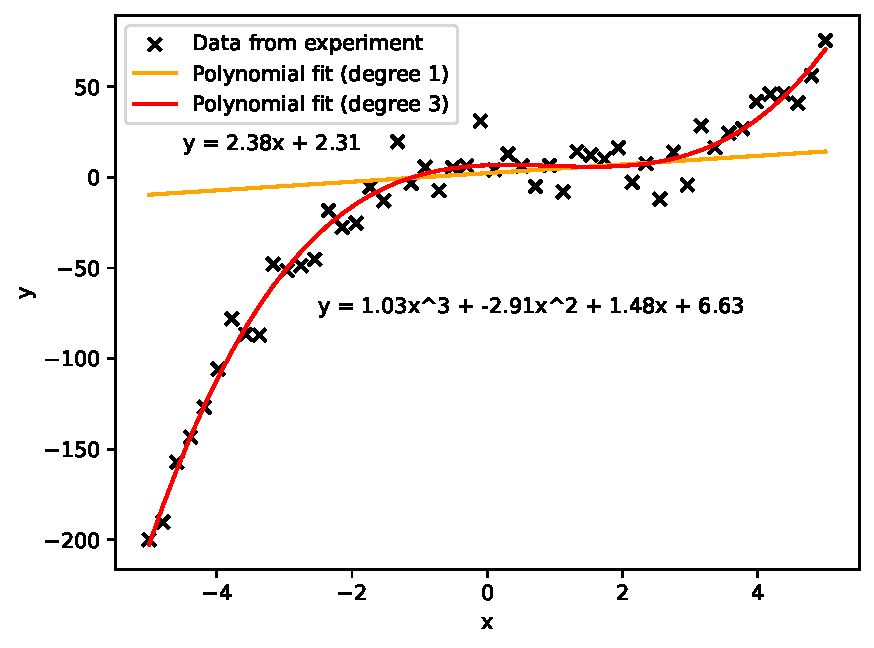
\includegraphics[width=\linewidth]{fig/fitting3.pdf}
\end{minipage}
\end{frame}

\begin{frame}
  \frametitle{Fitting Data - Uncertainty}
  Every measurement has it's own uncertainty.\\ We add uncertainty-bars to the data points using the \hrefu{https://matplotlib.org/stable/api/_as_gen/matplotlib.pyplot.errorbar.html}{\texttt{errorbar()}} function:
  \lstinputlisting[language=python, firstline=10,lastline=11]{examples/fitting3.py}
  First two arguments are the data, \texttt{yerr} and \texttt{xerr} are the uncertainties. \texttt{color} specifies the color of the datapoints and \texttt{ecolor} the color of the errorbars.
\end{frame}

\begin{frame}
  \frametitle{Fitting Data - Uncertainty}
  \begin{figure}[H]
    \centering
    \begin{samepage}
        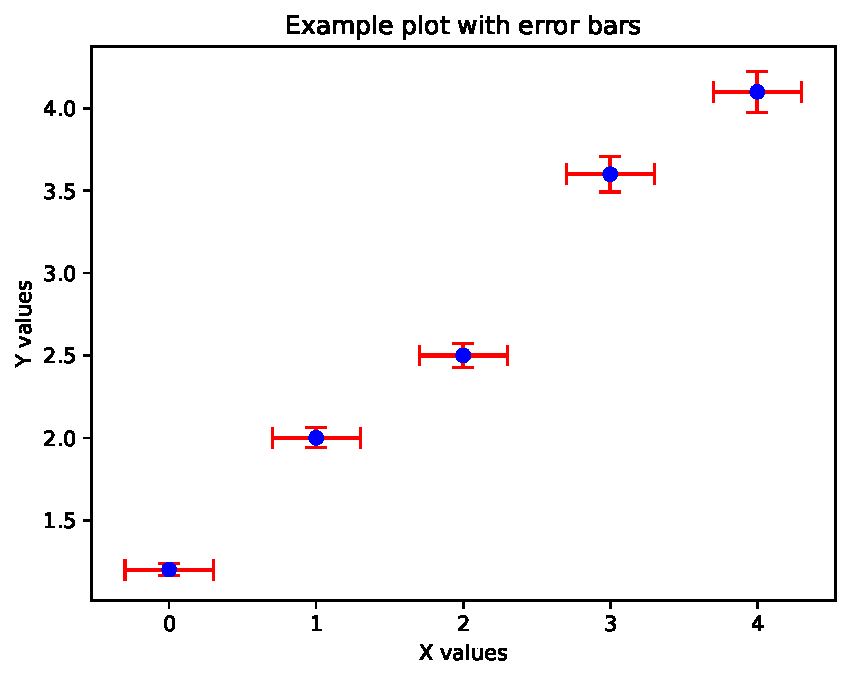
\includegraphics[width=0.65\linewidth]{fig/fitting4.pdf}
    \end{samepage}
\end{figure}
\end{frame}
%%%%%%%%%%%%%%%%%%%%%%%%%%%%%%%%%%%%%%%%%%%%%%%%%%%%%%%%%%%%%%%%%%%%%%%%%%%%
\end{document}
%%%%%%%%%%%%%%%%%%%%%%%%%%%%%%%%%%%%%%%%%%%%%%%%%%%%%%%%%%%%%%%%%%%%%%%%%%%%

%% EOF
